Question on point group symmetries and their consequences.

\begin{parts}
	\part Sketch of the direct lattice and its symmetry elements:
	\begin{figure}[H]
		\centering
		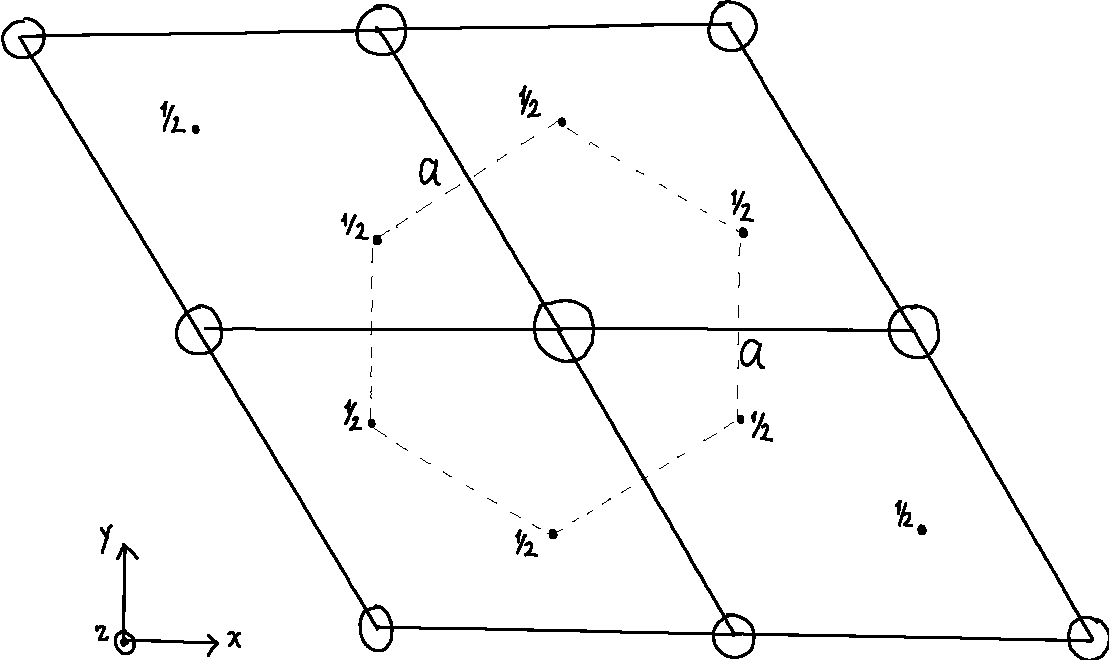
\includegraphics[width=.8\linewidth]{q4-direct-lattice}
		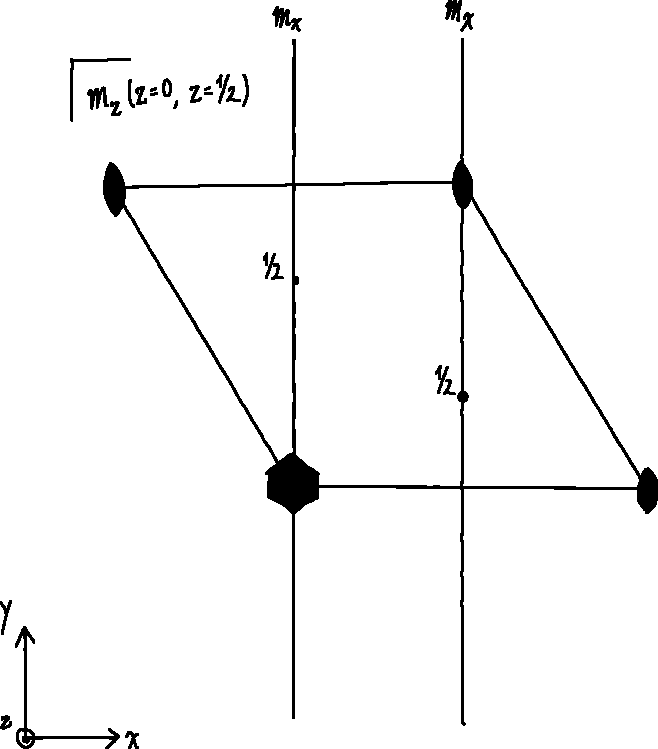
\includegraphics[width=.55\linewidth]{q4-symmetry-elements}
	\end{figure}
	Noting the {\varhexagon} structure due to $a = b$, we have the highest rotational symmetry of $6_z$.
	$2_z$ through the Mg atoms.
	$m_z$ at $z = 0$ and $z = 1/2$.
	$m_x$ through the B atoms.
	We also have $\bar{1}$ present at the centre $(1/2, 1/2, 1/2)$.
	
	\part We find the reciprocal lattice vector by definition:
	\begin{align*}
		\mathbf{a}^* &= 2\pi \frac{\mathbf{b} \times \mathbf{c}}{\mathbf{a \cdot \left(\mathbf{b} \times \mathbf{c}\right)}} \Rightarrow \mathbf{a}^* \textnormal{ $30\degree$ from $\mathbf{a}$} \\
		\mathbf{b}^* &\propto \mathbf{c} \times \mathbf{a} \Rightarrow \mathbf{b}^* \textnormal{ $-30\degree$ from $\mathbf{b} \Rightarrow \hat{\mathbf{y}}$}
	\end{align*}
	
	Sketch of the reciprocal lattice:
	\begin{figure}[H]
		\centering
		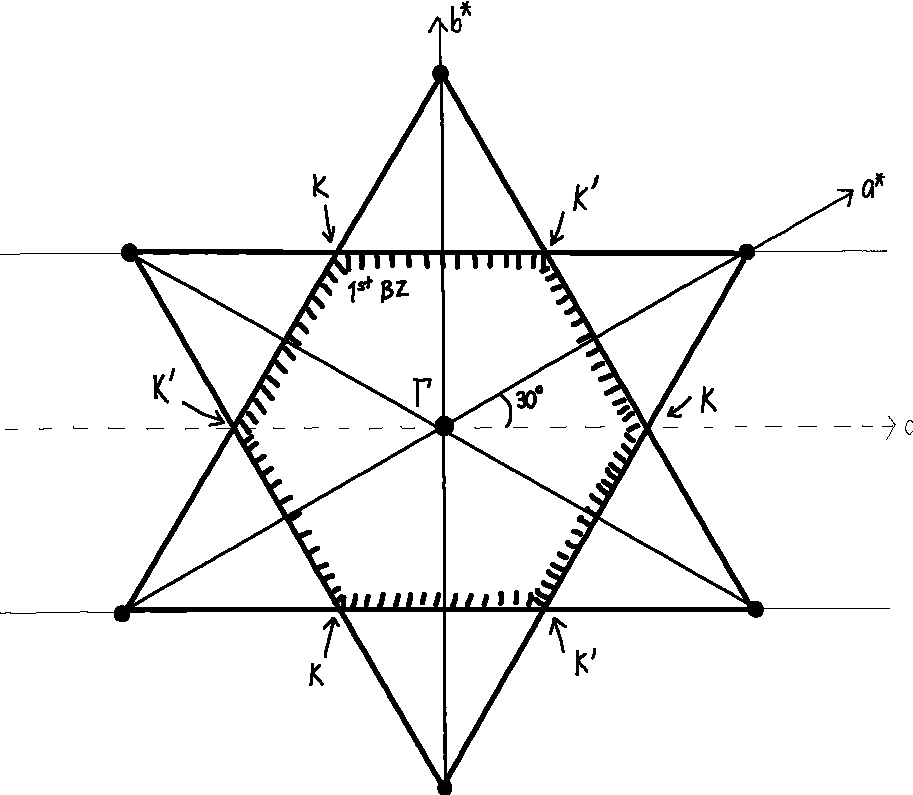
\includegraphics[width=.8\linewidth]{q4-reciprocal-lattice}
	\end{figure}
	
	\part Character table ($p_i$ is polarisation along $i$):
	
	\begin{center}
		\begin{tabular}{c|>{\columncolor{grey}}c|c|c|c|>{\columncolor{grey}}c}
		 & A & B & $p_x$ & $p_y$ & $p_z$ \\
		 \hline
		 $\bar{1}$ & -1 & -1 & -1 & -1 & -1 \\
		 $2_z$ & +1 & -1 & -1 & -1 & +1 \\
		 $m_z$ & -1 & -1 & +1 & +1 & -1 \\
		 $m_x$ & +1 & -1 & -1 & +1 & +1
		\end{tabular}
	\end{center}
	
	So only mode A is IR active with polarisation along $z$.
	
	\newpage
	
	\part Sketch of the reciprocal lattice points again:
	\begin{figure}[H]
		\centering
		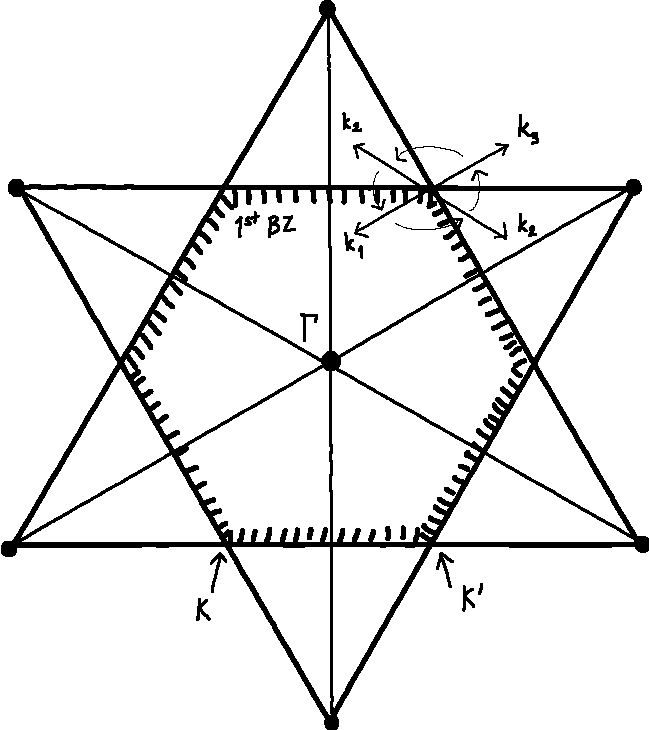
\includegraphics[width=.6\linewidth]{q4-k-degeneracy}
	\end{figure}
	Note that within $\Gamma$ point, all wavevectors within the 1st BZ remain inside after $3_z$ about $\Gamma$.
	However, for K there is a mixing between 1st and 2nd BZ (see the sketch above), which carries a phase of $\pi$ $\Rightarrow$ thus A and B are degenerate about K by symmetry.
\end{parts}